\documentclass[a4]{article}
\pagestyle{myheadings}

%%%%%%%%%%%%%%%%%%%
% Packages/Macros %
%%%%%%%%%%%%%%%%%%%
\usepackage{mathrsfs}


\usepackage{fancyhdr}
\pagestyle{fancy}
\lhead{}
\chead{}
\rhead{}
\lfoot{}
\cfoot{} 
\rfoot{\normalsize\thepage}
\renewcommand{\headrulewidth}{0pt}
\renewcommand{\footrulewidth}{0pt}
\newcommand{\RomanNumeralCaps}[1]
    {\MakeUppercase{\romannumeral #1}}

\usepackage{amssymb,latexsym}  % Standard packages
\usepackage[utf8]{inputenc}
\usepackage[russian]{babel}
\usepackage{MnSymbol}
\usepackage{mathrsfs}
\usepackage{amsmath,amsthm}
\usepackage{indentfirst}
\usepackage{graphicx}%,vmargin}
\usepackage{graphicx}
\graphicspath{{pictures/}} 
\usepackage{verbatim}
\usepackage{color}
\usepackage[nottoc,numbib]{tocbibind}
\usepackage{float}

\usepackage{listings}
\definecolor{codegreen}{rgb}{0,0.6,0}
\definecolor{codegray}{rgb}{0.5,0.5,0.5}
\definecolor{codepurple}{rgb}{0.58,0,0.82}
\definecolor{backcolour}{rgb}{0.95,0.95,0.92}
 
\lstdefinestyle{mystyle}{
    backgroundcolor=\color{backcolour},   
    commentstyle=\color{codegreen},
    keywordstyle=\color{magenta},
    numberstyle=\tiny\color{codegray},
    stringstyle=\color{codepurple},
    basicstyle=\footnotesize,
    breakatwhitespace=false,         
    breaklines=true,                 
    captionpos=b,                    
    keepspaces=true,                 
    numbers=left,                    
    numbersep=5pt,                  
    showspaces=false,                
    showstringspaces=false,
    showtabs=false,                  
    tabsize=2
}
 
\lstset{style=mystyle}

\usepackage{url}
\urldef\myurl\url{foo%.com}





\DeclareGraphicsExtensions{.pdf,.png,.jpg}% -- настройка картинок

\usepackage{epigraph} %%% to make inspirational quotes.
\usepackage[all]{xy} %for XyPic'a
\usepackage{color} 
\usepackage{amscd} %для коммутативных диграмм
%\usepackage[colorlinks,urlcolor=red]{hyperref}

%\renewcommand{\baselinestretch}{1.5}
%\sloppy
%\usepackage{listings}
%\lstset{numbers=left}
%\setmarginsrb{2cm}{1.5cm}{1cm}{1.5cm}{0pt}{0mm}{0pt}{13mm}


\newtheorem{Lemma}{Лемма}[section]
\newtheorem{Proposition}{Предложение}[section]
\newtheorem{Theorem}{Теорема}[section]
\newtheorem{Corollary}{Следствие}[section]
\newtheorem{Remark}{Замечание}[section]
\newtheorem{Definition}{Определение}[section]
\newtheorem{Designations}{Обозначение}[section]




%%%%%%%%%%%%%%%%%%%%%%% 
%Подготовка оглавления% 
%%%%%%%%%%%%%%%%%%%%%%% 
\usepackage[titles]{tocloft}
\renewcommand{\cftdotsep}{2} %частота точек
\renewcommand\cftsecleader{\cftdotfill{\cftdotsep}}
\renewcommand{\cfttoctitlefont}{\hspace{0.38\textwidth} \LARGE\bfseries} 
\renewcommand{\cftsecaftersnum}{.}
\renewcommand{\cftsubsecaftersnum}{.}
\renewcommand{\cftbeforetoctitleskip}{-1em} 
\renewcommand{\cftaftertoctitle}{\mbox{}\hfill \\ \mbox{}\hfill{\footnotesize Стр.}\vspace{-0.5em}} 
%\renewcommand{\cftchapfont}{\normalsize\bfseries \MakeUppercase{\chaptername} } 
%\renewcommand{\cftsecfont}{\hspace{1pt}} 
\renewcommand{\cftsubsecfont}{\hspace{1pt}} 
%\renewcommand{\cftbeforechapskip}{1em} 
\renewcommand{\cftparskip}{3mm} %определяет величину отступа в оглавлении
\setcounter{tocdepth}{5} 
\renewcommand{\listoffigures}{\begingroup %добавляем номер в список иллюстраций
\tocsection
\tocfile{\listfigurename}{lof}
\endgroup}


   
   
%\renewcommand{\thelikesection}{(\roman{likesection})}
%%%%%%%%%%%
% Margins %
%%%%%%%%%%%
\addtolength{\textwidth}{0.7in}
\textheight=630pt
\addtolength{\evensidemargin}{-0.4in}
\addtolength{\oddsidemargin}{-0.4in}
\addtolength{\topmargin}{-0.4in}

%%%%%%%%%%%%%%%%%%%%%%%%%%%%%%%%%%%
%%%%%%Переопределение chapter%%%%%% 
%%%%%%%%%%%%%%%%%%%%%%%%%%%%%%%%%%%
\newcommand{\empline}{\mbox{}\newline} 
\newcommand{\likechapterheading}[1]{ 
\begin{center} 
\textbf{\MakeUppercase{#1}} 
\end{center} 
\empline} 

%%%%%%%Запиливание переопределённого chapter в оглавление%%%%%% 
\makeatletter 
\renewcommand{\@dotsep}{2} 
\newcommand{\l@likechapter}[2]{{\bfseries\@dottedtocline{0}{0pt}{0pt}{#1}{#2}}} 
\makeatother 
\newcommand{\likechapter}[1]{ 
\likechapterheading{#1} 
\addcontentsline{toc}{likechapter}{\MakeUppercase{#1}}} 




\usepackage{xcolor}
\usepackage{hyperref}
\definecolor{linkcolor}{HTML}{000000} % цвет ссылок
\definecolor{urlcolor}{HTML}{AA1622} % цвет гиперссылок
 
\hypersetup{pdfstartview=FitH,  linkcolor=linkcolor,urlcolor=urlcolor, colorlinks=true}

%%%%%%%%%%%%
% Document %
%%%%%%%%%%%%

%%%%%%%%%%%%%%%%%%%%%%%%%%%%%
%%%%%%главы -- section*%%%%%%
%%%%section -- subsection%%%%
%subsection -- subsubsection%
%%%%%%%%%%%%%%%%%%%%%%%%%%%%%
\def \newstr {\medskip \par \noindent} 



\begin{document}
\def\contentsname{\LARGE{Содержание}}
\thispagestyle{empty}
\begin{center} 
\vspace{2cm} 
{\Large \sc Санкт-Петербургский Политехнический}\\
\vspace{2mm}
{\Large \sc Университет} им. {\Large\sc Петра Великого}\\
\vspace{1cm}
{\large \sc Институт прикладной математики и механики\\ 
\vspace{0.5mm}
\textsc{}}\\ 
\vspace{0.5mm}
{\large\sc Кафедра прикладной математики}\\
\vspace{15mm}
%\rule[0.5ex]{\linewidth}{2pt}\vspace*{-\baselineskip}\vspace*{3.2pt} 
%\rule[0.5ex]{\linewidth}{1pt}\\[\baselineskip] 
{\huge \sc Лабораторная работа №$2$\\
\vspace{0.1cm}
Характеристики положения\\
\vspace{0.5cm}
выборки
\vspace{6mm}
 }
\vspace*{2mm}
%\rule[0.7ex]{\linewidth}{1pt}\vspace*{-\baselineskip}\vspace{3.2pt} 
%\rule[0.5ex]{\linewidth}{2pt}\\ 
\vspace{1cm}

{\sc $3$ курс$,$ группа $33631/2$}

\vspace{2cm} 
Студент \hfill Д. А. Плаксин\\
\vspace{1cm}
Преподаватель \hfill Баженов А. Н.\\
\vspace{20mm} 

\end{center} 
%\author{Я}
\begin{center}
\vfill {\large\textsc{Санкт-Петербург}}\\ 
2019 г.
\end{center}

%%%%%%%%%%%%%%%%%%%%%%%%%%%%%%%%%%%%%%%%%%%%%%%%%%%%%%%%%%%%%%%%%%%%%%%%%%%%%%%%%%%%%%%%%%%%%%
%\ \\[4cm]

%\rm
%%%%%%%%%%%%%%%%%%%%%%%%%%%%%%%%%%%%%%%%%%%%%%%%%%%%%%%%%%%%%%%%%%%%%%%%%%%%%%%%%%%%%%%%%%%%%%
\newpage
\pagestyle{plain}

%\begin{center}
%\begin{abstract} 

%\end{abstract}

%\end{center}

\newpage
\tableofcontents{}
\newpage
\listoffigures
\newpage

\section{Постановка задачи}

Любыми средствами сгенерировать выборки размеров $20,$ $60,$ $100$ элементов для $5$ти распределений \cite{distr_formulas}. Для каждой выборки вычислить $\overline{x},\; med\; x,\; Z_R,\; Z_Q,\; Z_{tr},$ при $r = \frac{n}{4}.$

Распределения:
\begin{enumerate}
\item Стандартное нормальное распределение
\item Стандартное распределение Коши
\item Распределение Лапласа с коэффициентом масштаба $\sqrt{2}$ и нулевым коэффициентом сдвига.
\item Равномерное распределение на отрезке $\left[-\sqrt{3}, \sqrt{3}\right]$
\item Распределение Пуассона со значением матожидания равным двум.
\end{enumerate}

\begin{comment}
\begin{equation}\label{eqn:normal}
N(x,0,1) = \frac{1}{\sqrt{2\pi}}e^{-\frac{x^2}{2}}
\end{equation} 

\begin{equation}\label{eqn:cauchy}
 C(x,0,1) = \frac{1}{\pi(1+x^2)}
 \end{equation}
 
 \begin{equation}\label{eqn:laplace}
 L\left( x,0,\frac{1}{\sqrt{2}}\right) = \frac{1}{\sqrt{2}}e^{-\sqrt{2}\vert x\vert}
 \end{equation}
 
 \begin{equation}\label{eqn:poisson}
 P(\lambda,k) = \frac{\lambda^k}{k!}e^{-\lambda}
\end{equation}  

\begin{equation}\label{eqn:uniform}
M(x,-\sqrt{3}, \sqrt{3}) = 
 \begin{cases}
   \frac{1}{2\sqrt{3}} &\vert x\vert \leqslant \sqrt{3}\\
   0 &\vert x\vert > \sqrt{3}
 \end{cases}
\end{equation}
\end{comment}

\section{Теория}

\begin{enumerate}
\item Выборочное среднее \cite{average}:
\begin{equation}\label{eqn:average}
\overline{x} = \frac{1}{n}\sum_{i=1}^n x_i \hfill  
\end{equation}
\item Выборочная медиана \cite{med}:
\begin{equation}
med\; x = \begin{cases}
x_{k+1}, & n = 2k+1\\
\frac{1}{2}\left(x_k+x_{k+1}\right), & n = 2k
\end{cases} \hfill  \label{eqn:med}
\end{equation}
\item Полусумма экстремальных значений \cite{mean_extr}:
\begin{equation}
Z_R = \frac{1}{2}\left(x_1+x_n\right) \hfill  \label{eqn:mean_extr}
\end{equation}
\item Полусумма квартилей \cite{quartiles}:
\begin{equation}
Z_Q = \frac{1}{2}\left(Z_{\frac{1}{4}}+Z_{\frac{3}{4}}\right) \hfill  \label{eqn:quartiles}
\end{equation}
\item Усечённое среднее \cite{cut_mean}:
\begin{equation}
Z_{tr} = \frac{1}{n - 2r}\sum_{i=r+1}^{n-r} x_i \hfill  \label{eqn:cut_mean}
\end{equation}
\end{enumerate}

\section{Реализация}
Для генерации выборки был использован $Python\;3.7$: модуль $random$ библиотеки $numpy$ \cite{numpy} для генерации случайных чисел с различными распределениями. Также с помощью библиотеки $numpy$ были вычислены характеристики положения.

После вычисления характеристик положения $1000$ раз находится среднее значение и дисперсия: $E(z) = \frac{1}{n}\sum_{i=1}^n z_i,\; D(z) = E\left(z^2\right) - E^2(z).$

\newpage
\section{Результаты}

\begin{figure}[H]
  \centering
  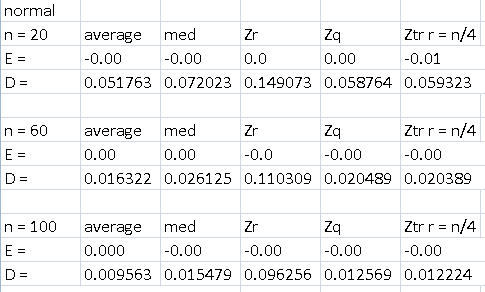
\includegraphics[width=\textwidth]{normalFix.png}
  \caption{Стандартное нормальное распределение:}
\end{figure}

\begin{figure}[H]
  \centering
  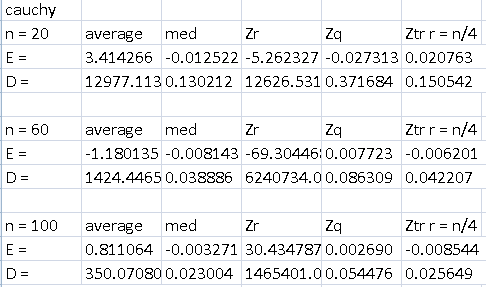
\includegraphics[width=\textwidth]{cauchy.png} 
  \caption{Стандартное распределение Коши}
\end{figure}

\begin{figure}[H]
  \centering
  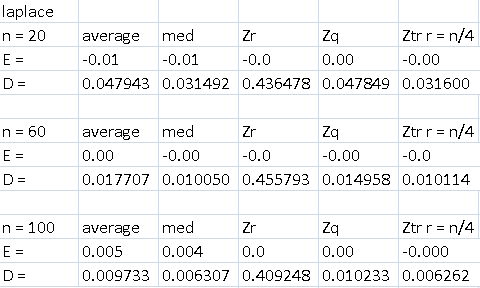
\includegraphics[width=\textwidth]{laplaceFix.png} 
  \caption{Распределение Лапласа}
\end{figure}

\begin{figure}[H]
  \centering
  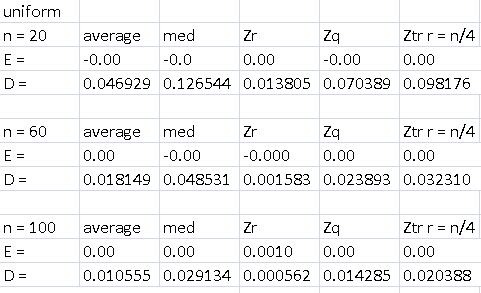
\includegraphics[width=\textwidth]{uniformFix.png}
  \caption{Равномерное распределение}
\end{figure}

\begin{figure}[H]
  \centering
  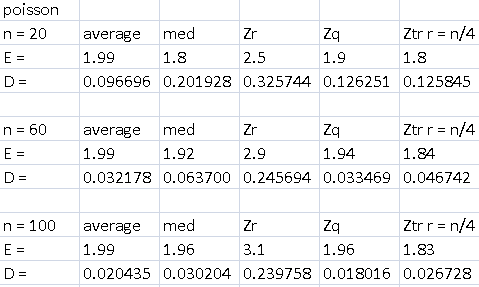
\includegraphics[width=\textwidth]{poissonFix.png} 
  \caption{Распределение Пуассона}
\end{figure}

\section{Обсуждение}
\par При вычислении средних значений пришлось отбрасывать некоторое число знаков после запятой, так как получаемая дисперсия не могла гарантировать получаемое точное значение. \par Иными словами дисперсия может гарантировать порядок точности среднего значения только до первого значащего знака после запятой в дисперсии включительно. \par Единственным исключением [в отбрасывании знаков после запятой] стало стандартное распределение Коши, так как оно имеет бесконечную дисперсию, а значит может гарантировать сколь угодно большую точность.

\section{Выводы}

\par В процессе работы вычислены значения характеристик положения для определённых распределений на выборках фиксированной мощности и получено следующее ранжирование характеристик положения:

\begin{enumerate}
    \item Стандартное нормальное распределение $$\overline{x} < Z_{tr} < Z_Q < med\;x < Z_R$$
    
    \item Стандартное распределение Коши $$med\;x < Z_Q < Z_{tr} < \overline{x} < Z_R$$
    
    \item Распределение Лапласа (коэффициент масштаба $\sqrt{2}$ коэффициент сдвига равен нулю) $$med\;x < Z_{tr} < \overline{x} < Z_Q < Z_R$$
    
    \item Равномерное распределение на отрезке $\left[-\sqrt{3},\sqrt{3}\right]$ $$Z_R < \overline{x} < Z_{tr} < Z_Q < med\;x$$
    
    \item Распределение Пуассона (значение мат ожидания равно $3$) $$\overline{x} < Z_{tr} < Z_Q < med\;x < Z_R$$
    
\end{enumerate}



\begin{thebibliography}{}
    \bibitem{numpy}  Модуль numpy  -  https://physics.susu.ru/vorontsov/language/numpy.html
    
    \bibitem{distr_formulas}  
    Формулы распределений  -  https://vk.com/doc184549949\_491827451
    
    \bibitem{average}  
    Выборочное среднее  -  https://en.wikipedia.org/wiki/Sample\_mean\_and\_covariance
    
    \bibitem{med}  
    Выборочная медиана  -  http://femto.com.ua/articles/part\_1/2194.html
    
    \bibitem{mean_extr}  
    Полусумма экстремальных значений  -  https://studopedia.info/8-56888.html
    
    \bibitem{quartiles}  
    Квартили  -  https://studfiles.net/preview/2438125/page:13/
    
    \bibitem{cut_mean}  Усечённое среднее  -  https://ole-olesko.livejournal.com/15773.html
\end{thebibliography}

\section{Приложения}

 
Код отчёта:\; \url{https://github.com/MisterProper9000/MatStatLabs/blob/master/MatStatLab2/MatStatLab2.tex}

Код лаборатрной:\; \url{https://github.com/MisterProper9000/MatStatLabs/blob/master/MatStatLab2/MatStatLab2.py}

\lstinputlisting[language=Python]{MatStatLab2.py}

\end{document}
